%________________________________________________________________________________________________
\documentclass{beamer}
%________________________________________________________________________________________________
\usepackage[french]{babel} 
\usepackage[utf8]{inputenc} 
\usepackage[T1]{fontenc} 
\usepackage{graphicx}
\usepackage[utf8]{inputenc}
\usepackage{fancyhdr}
\usepackage{geometry}
\usepackage{tabularx,tabulary}
\usepackage{movie15}
%________________________________________________________________________________________________
\title{3I013 Réunion du 29 Mars 2019}
\author{Nicolas CASTANET\\Maël FRANCESCHETTI\\Daoud KADOCH\\Fabien MANSON\\}
%________________________________________________________________________________________________
%ce theme est le plus clean de Beamer le truc a ne pas utiliser c'est 'Warsaw'
\usetheme{default}
%suppression de la barre de navigation inutile
\setbeamertemplate{navigation symbols}{}
\setbeamertemplate{frametitle}[default][center]

%\logo{
\includegraphics[height=0.5cm]{logo_sorbonne.png}}

%________________________________________________________________________________________________
\addtobeamertemplate{footline}{
	\begin{flushright}
	\vbox{\insertframenumber/\inserttotalframenumber}
	\end{flushright}}

%________________________________________________________________________________________________
\begin{document}


	\begin{frame}
		\begin{center}
		\date{}
		\maketitle
		\end{center}
	\end{frame}
	
	
	
	\begin{frame}
		\section{}
		\begin{center}
		\frametitle{Sommaire}
		\tableofcontents{}
		\end{center}
	\end{frame}
	
	
	
	\begin{frame}
		\section{Contexte}
		\begin{center}
		\frametitle{L'Objectif du Projet}
		   Faire effectuer une ronde à un drone Bebop 2 en suivant un itinéraire prédéfini, tout en visualisant le retour vidéo en temps réel sur un iPod à travers un masque FPV.
		\end{center}
	\end{frame}
	
	
	
	\begin{frame}
		\section{Architecture Logicielle Complète}
		\begin{center}
		\frametitle{Architecture Logicielle}
		%\subsection{Contraintes}
        %\framesubtitle{Les solutions}
       
        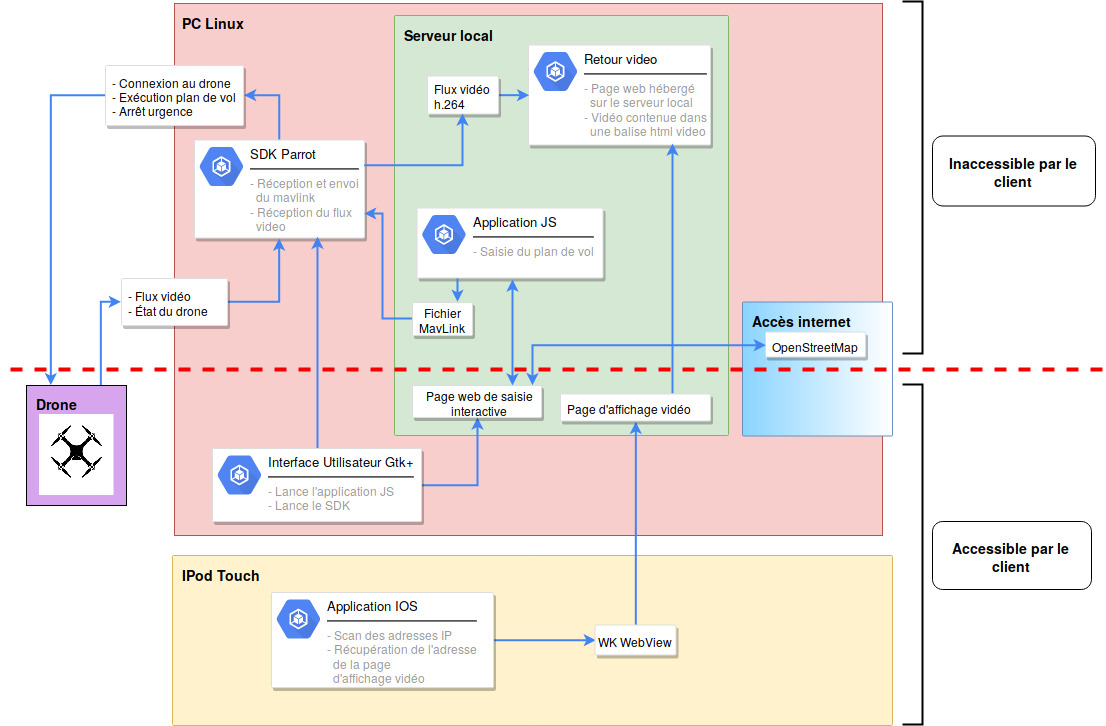
\includegraphics[scale=0.3]{Architecture_logicielle_composants/Architecture_logicielle_v2.jpg}
		\end{center}
	\end{frame}
	
	
	
	\begin{frame}
		\section{SDK Parrot}
		\begin{center}
		\frametitle{SDK Parrot}
		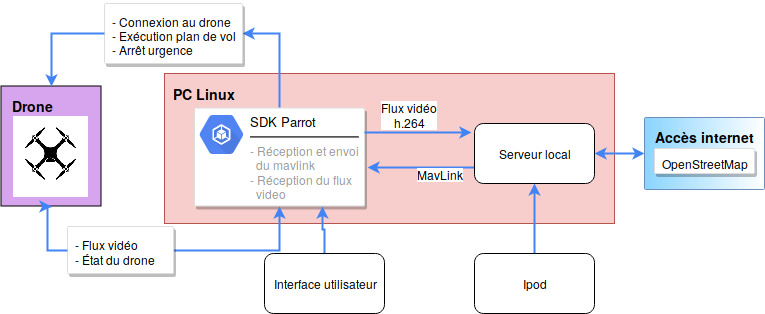
\includegraphics[scale=0.4]{Architecture_logicielle_composants/SDK.jpg}
		\end{center}	
	\end{frame}
	
	
	
	\begin{frame}
		\section{Serveur local}
		\begin{center}
		\frametitle{Serveur local}
		%\subsection{Contraintes}
        %\framesubtitle{Les solutions}
        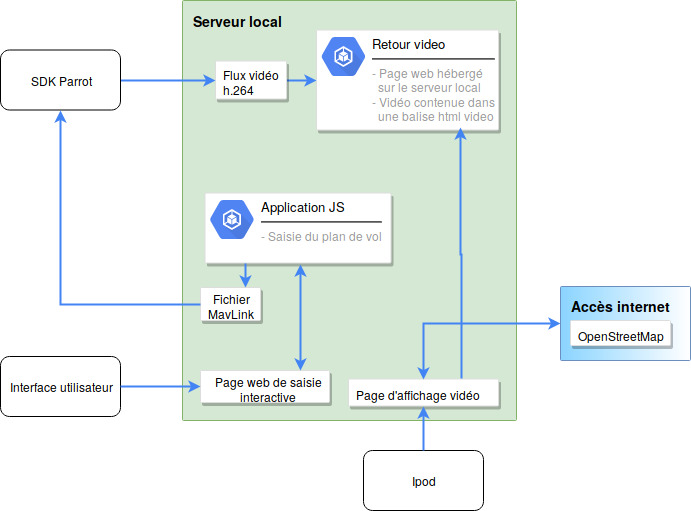
\includegraphics[scale=0.4]{Architecture_logicielle_composants/Serveur.jpg}
		\end{center}
	\end{frame}
	
	
	
	\begin{frame}
		\section{Application iOS}
		\begin{center}
		\frametitle{Application iOS}
        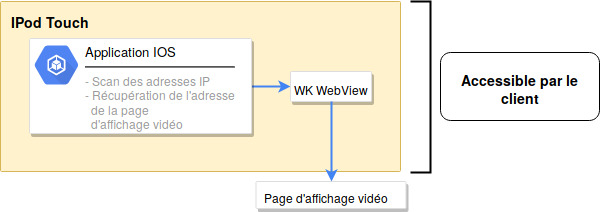
\includegraphics[scale=0.5]{Architecture_logicielle_composants/ios_app.jpg}
		\end{center}
	\end{frame}
	
	
	
	\begin{frame}
		\section{Application iOS}
		\begin{center}
		\frametitle{Application iOS}
        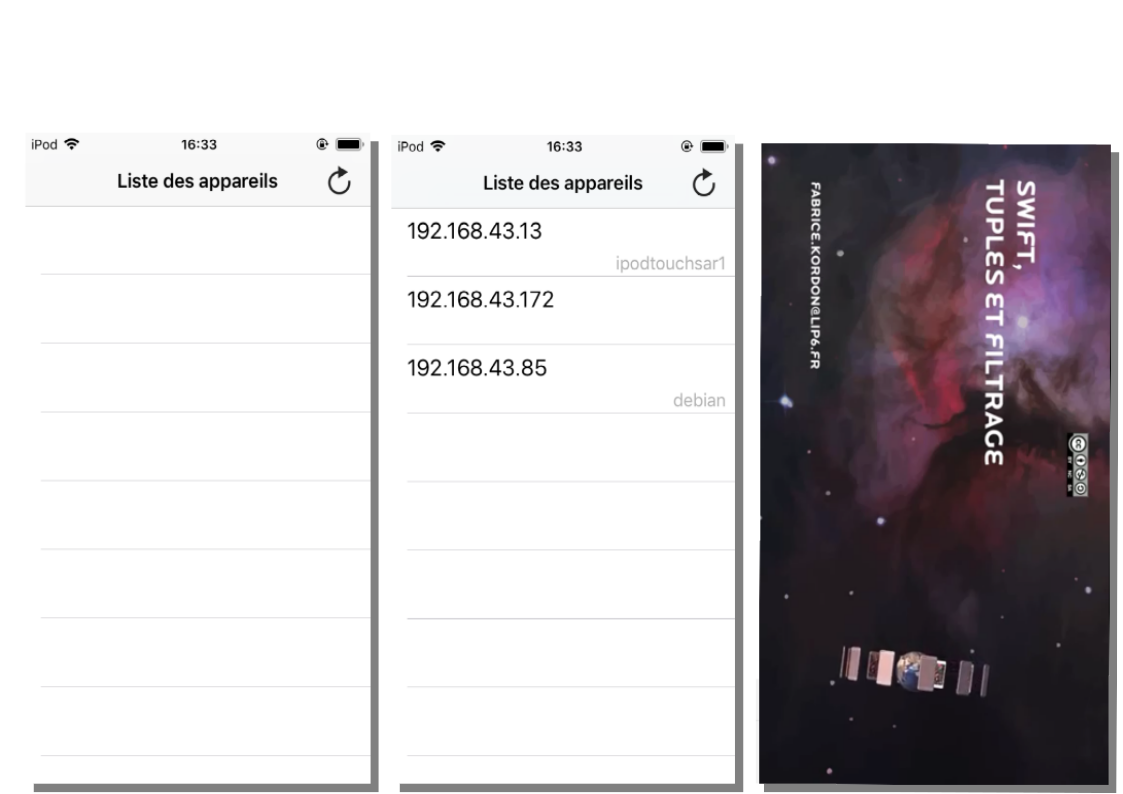
\includegraphics[scale=0.37]{Architecture_logicielle_composants/ipod.png}
		\end{center}
	\end{frame}
	
	
	
	\begin{frame}
		\section{Interface Utilisateur}
		\begin{center}
		\frametitle{Interface Utilisateur}
		%\subsection{Contraintes}
        %\framesubtitle{Les solutions}
        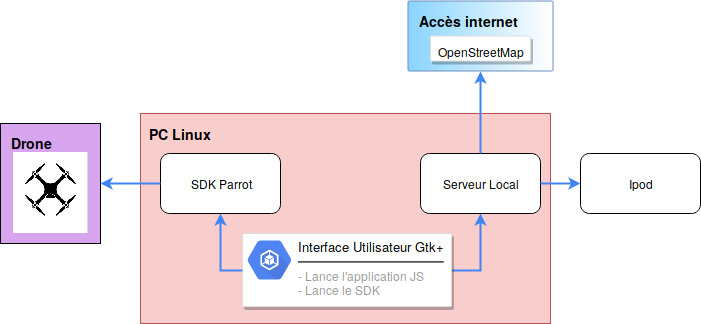
\includegraphics[scale=0.4]{Architecture_logicielle_composants/Interface_utilisateur.jpg}
		\end{center}
	\end{frame}
	
	
	
	\begin{frame}
		\frametitle{Interface GTK+}
		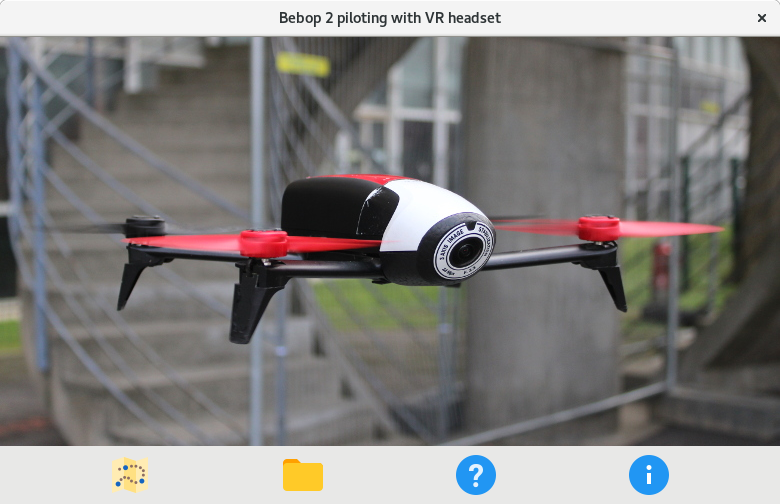
\includegraphics[scale=0.4]{Architecture_logicielle_composants/GUI-v2.png}	
	
	\end{frame}
	
	
	\begin{frame}
		\section{Tests}
		\begin{center}
		\frametitle{Tests effectués}
           	\begin{itemize}
                \item Connexion au drone.
                \item Envoi d'un fichier Mavlink avec le SDK.
                \item Exécution du plan de vol enregistré sur le drone (jamais dans sa totalité).
                \item Retour vidéo avec l'application iOS à partir d'une url sur un serveur local Linux.
            \end{itemize}
		\end{center}
	\end{frame}
	
	
	
	\begin{frame}
		\begin{center}
		\frametitle{Problèmes rencontrés}
             \begin{itemize}
                \item Calibration du drone après chaque arrêt d'urgence (choc ou inclinaison trop forte du drone).
                \item Perte du signal GPS (vol stationnaire).
                \item Direction du drone durant le trajet.
                \item Lecture d'un double flux vidéo sur. l'iPod.
            \end{itemize}
		\end{center}
	\end{frame}
	
	
\end{document}